\chapter{The Application Programming Interface}
\label{API}
	\section{Introduction}
		In this section we will briefly discuss the commnunication protocol used by the application to its internal components. The protocol used as mentioned
		already in the previous chapters, is a designed stateful[\cite{session-rfc6265}], Json-based[\cite{json-rfc7159}] Https[\cite{rfc2818}] RESTFull[\cite{restful-rfc7231}]
		protocol. Let us explain briefly what those techical terms mean.
		\subsection{Stateful Protocol}
			Stateful protocol[\cite{session-rfc6265}] is a protocol capable of recognising and distinquishing between the different requests made by the same host machine. 
			In our application this is essential because the authentication functionality would be impossible otherwise. An authenticated user is 
			always ascosiated with a sessionID. The sessionID[\cite{sessionID-rfc7329}] is a character string that is returned after the authentication is 
			complete and should be attached to every subsequent request for user authentication to work. Our application protocol uses the cookie mechanism
			to attach the sessionID to every request, ensuring that the Services will recognise the sender. The following image provides an example
			\begin{figure}[H]
				\iftrue
				\caption{Session ID Attached to Notifications Request, captured using Firefox-Tools}
				\centering
				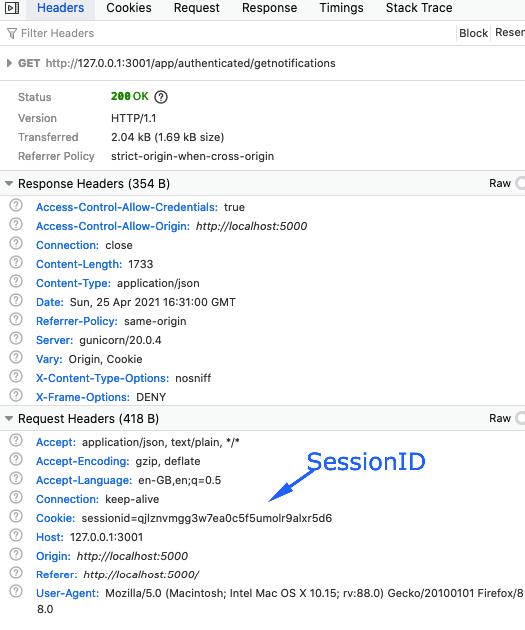
\includegraphics[scale=0.3]{figures/sessionID}
				\fi
			\end{figure} 
			Here, the Session ID is attached to a request from the Frontend Application into the Information Service, for the retrieval of new notifications
		\subsection{Json}
			The JavaScript Object Notation (or JSON) Data Interchange Format[\cite{json-rfc7159}] is a text-based, lightweight, human-readable language-indepedent
			data exchange format. We use JSON extensively to design our communication protocol, mainly because of his widely adopted use and availability of
			decoders. Additionally, both languages involved in the data transaction(javascript for the frontend, python for the backend services) are supporting
			JSON natively.
			\begin{figure}[H]
				\iftrue
				\caption{Capturing the Information service's JSON-Based responce using Postman}
				\centering
				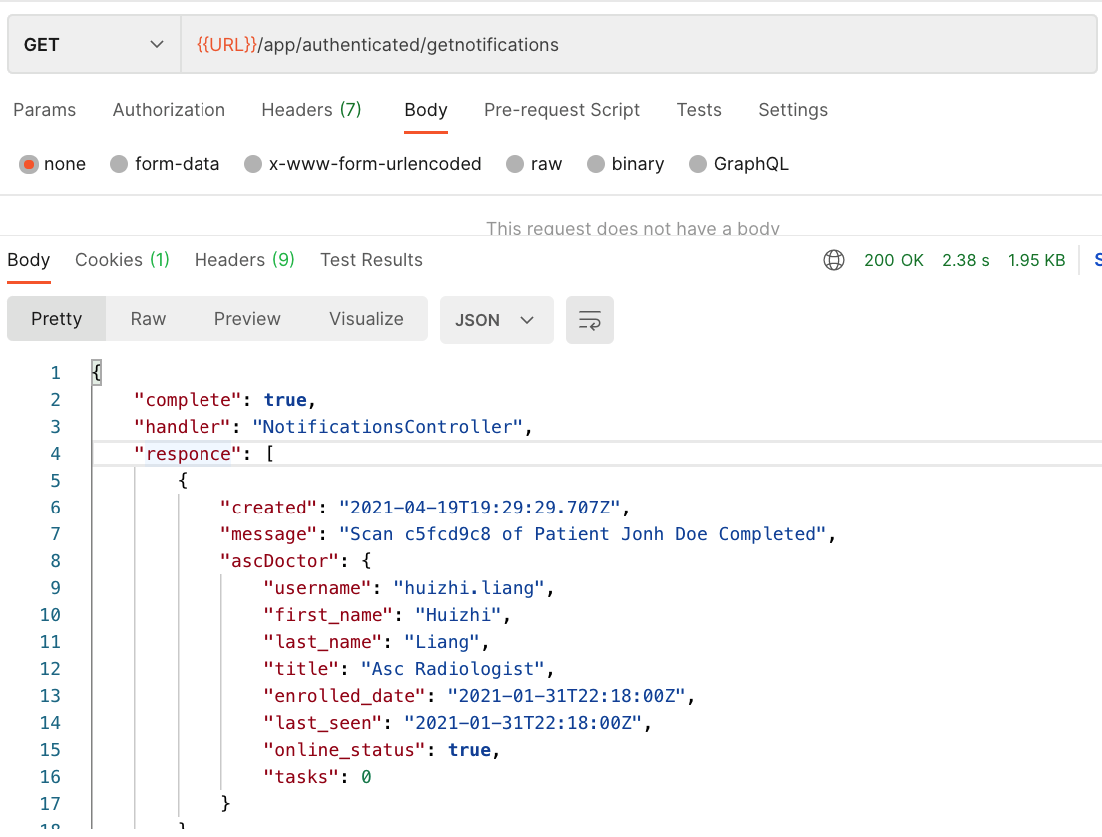
\includegraphics[scale=0.3]{figures/json}
				\fi
			\end{figure} 
		\subsection{HTTPS}
			HTTPS or HyperText Transfer Protocol Secure version, is a updated version of classic HTTP protocol, using TLS as an additional security layer. TLS 
			encrypts all the underlying data to provide unparallel protection against various malicious attacks. The following images shown the login packages as
			they sent from the Frontend Application to the Information Service using the WireShark packet analyser.
			\begin{figure}[H]
				\iftrue
				\caption{Unecrupted Credentials (HTTPS disabled)}
				\centering
				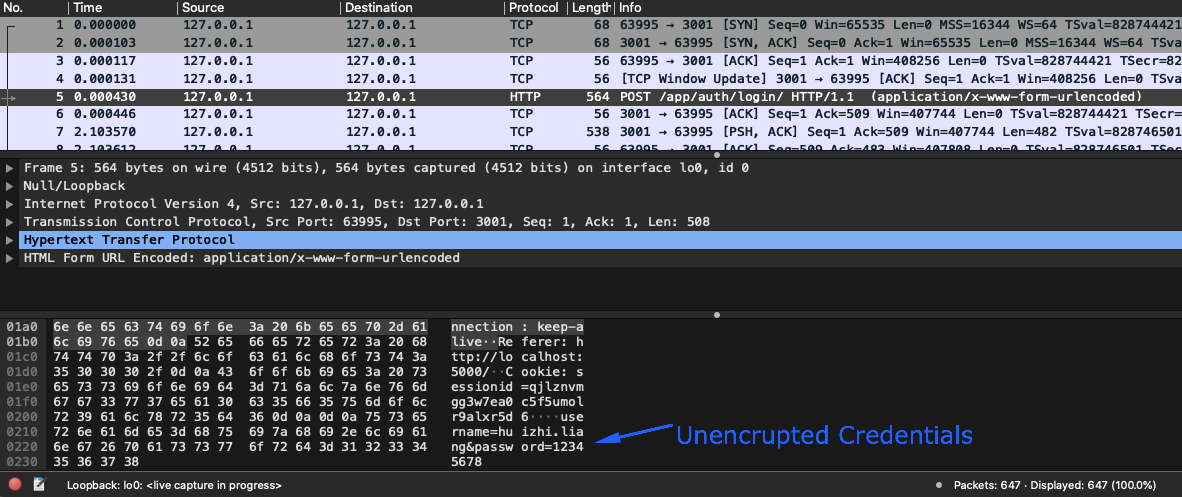
\includegraphics[scale=0.3]{figures/http}
				\fi
			\end{figure}
			\begin{figure}[H]
				\iftrue
				\caption{Ecrupted Credentials (HTTPS enabled)}
				\centering
				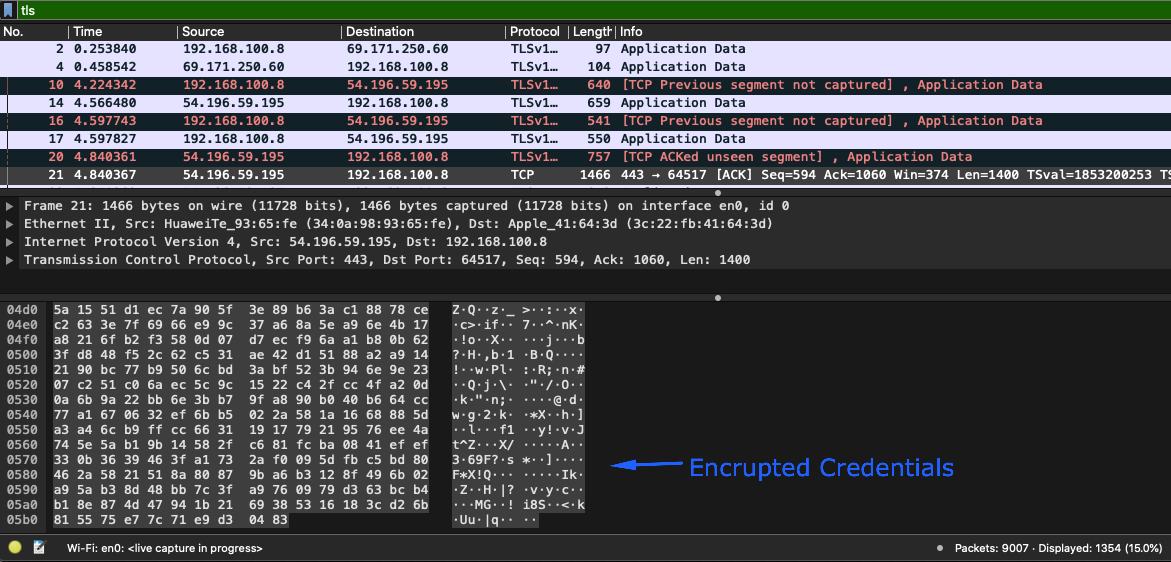
\includegraphics[scale=0.3]{figures/https}
				\fi
			\end{figure}
			Becomes evident that, by using HTTPS we increase our system security, as credentials and personal information are encrupted before sent over the
			internet.
		\subsection{RESTFull protocol}
			
